% Created 2025-01-28 di 10:56
% Intended LaTeX compiler: pdflatex
\documentclass[bigger]{beamer}
\usepackage[utf8]{inputenc}
\usepackage[T1]{fontenc}
\usepackage{graphicx}
\usepackage{longtable}
\usepackage{wrapfig}
\usepackage{rotating}
\usepackage[normalem]{ulem}
\usepackage{amsmath}
\usepackage{amssymb}
\usepackage{capt-of}
\usepackage{hyperref}
\usepackage{graphicx}
\usepackage[export]{adjustbox}
\usepackage{hyperref}
\usepackage[normalem]{ulem}
\usepackage{ragged2e}
\beamertemplatenavigationsymbolsempty
\usetheme{Madrid}
\usecolortheme{dolphin}
\setbeamertemplate{footline}{\hfill\vspace{1em}\insertframenumber{}\;\;\;\,}
\usepackage{tikz}
\usetheme{default}
\author{Jeroen van Riel}
\date{January 2025}
\title{Coordination of autonomous vehicles}
\hypersetup{
 pdfauthor={Jeroen van Riel},
 pdftitle={Coordination of autonomous vehicles},
 pdfkeywords={},
 pdfsubject={},
 pdfcreator={Emacs}, 
 pdflang={English}}
\usepackage{natbib}
\begin{document}

\maketitle
\begin{frame}[label={sec:org5de096c}]{Coordination of autonomous vehicles}
\begin{figure}
  \centering
  \href{https://arxiv.org/src/2311.07435v4/anc/Animation_4_-_Only_Cars,_Medium_load.mp4}{
    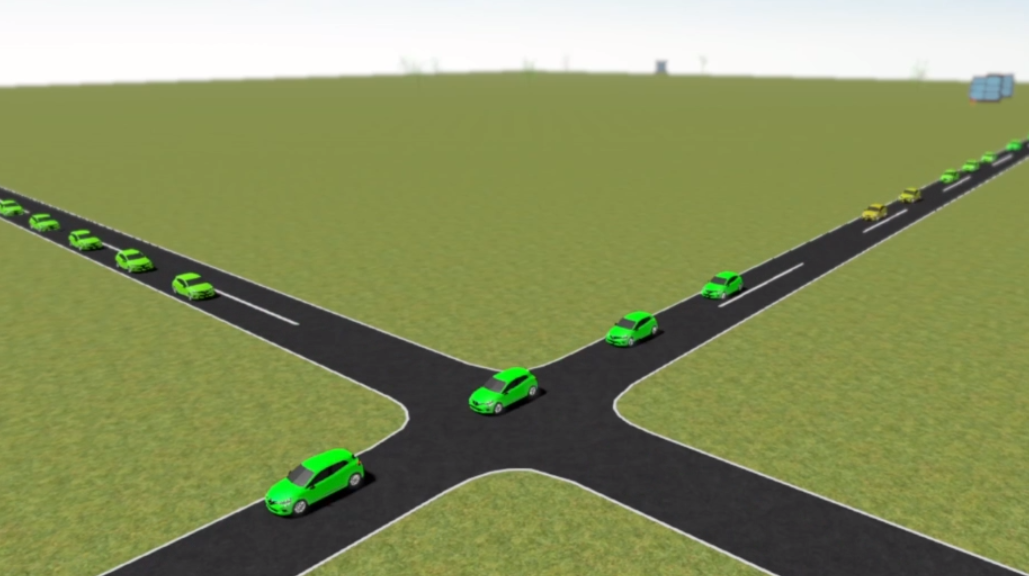
\includegraphics[width=0.55\textwidth]{figures/autonomous_simulation.png}
  }
\end{figure}

\(\vspace{0.1em}\)

\begin{itemize}
\item Less human intervention
\item Better guarantees on safety
\item Potentially reduce economic costs
\end{itemize}
\end{frame}
\begin{frame}[label={sec:org397b3fa}]{\ldots{}as optimal control problem}
\begin{tikzpicture}[remember picture, overlay]
\node[above=-6.5cm] at (current page.north)
{
  \href{https://github.com/jeroenvanriel/traffic-scheduling/blob/master/grid.gif}{
    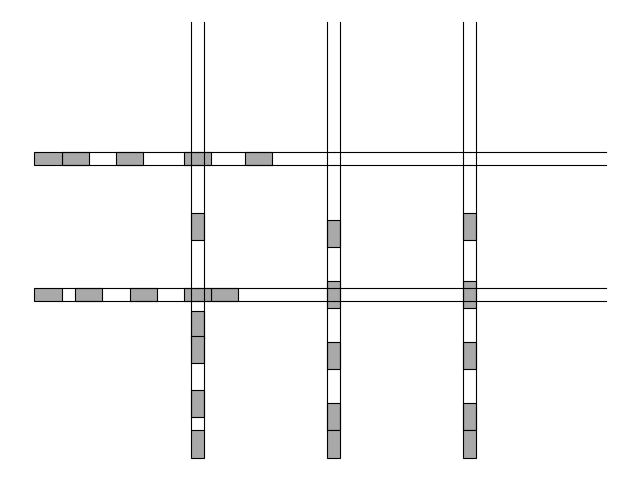
\includegraphics[width=0.55\textwidth]{figures/state_example.png}
  }
};
\end{tikzpicture}

\vspace{11.2em}

\begin{itemize}
\item Multi-agent optimal control problem
\begin{itemize}
\item Minimize total travel time
\item Avoid collisions
\end{itemize}
\end{itemize}
\end{frame}
\begin{frame}[label={sec:orgc4ab77a}]{\ldots{}as optimal control problem}
\begin{tikzpicture}[remember picture, overlay]
\node[above=-6.5cm] at (current page.north)
{
  \href{https://github.com/jeroenvanriel/traffic-scheduling/blob/master/grid.gif}{
    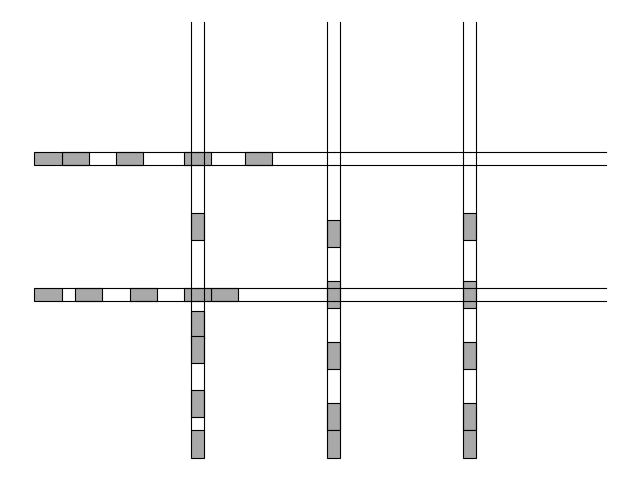
\includegraphics[width=0.55\textwidth]{figures/state_example.png}
  }
};
\end{tikzpicture}

\vspace{12em}

\begin{itemize}
\item Some initial assumptions
\begin{itemize}
\item Central control (with perfect communication)
\item Fixed routes
\item All future arrivals known
\end{itemize}
\end{itemize}
\end{frame}
\begin{frame}[label={sec:org3212957}]{How to solve it?}
\begin{itemize}
\item Direct transcription methods
\begin{itemize}
\item Solve as mixed-integer linear program
\item Provide optimal trajectories
\item Computationally very demanding
\end{itemize}
\end{itemize}

\(\vspace{0.1em}\)

\begin{itemize}
\item How to solve large instances?
\begin{itemize}
\item Need for approximation
\item Exploit problem structure (decomposition)
\item Automatically find heuristics (learning)
\end{itemize}
\end{itemize}
\end{frame}
\begin{frame}[label={sec:org916ca91}]{Research questions}
\setbeamercolor{block title}{use=structure,fg=structure.fg,bg=structure.fg!20!bg}
\setbeamercolor{block body}{parent=normal text,use=block title,bg=block title.bg!50!bg}

\begin{center}
  \begin{minipage}{0.8\textwidth}

\begin{block}{\small Q1: Decomposition}
\footnotesize \justifying How to model offline trajectory optimization
    as a variant of job-shop scheduling?
\end{block}
\begin{block}{\small Q2: Learning}
\footnotesize \justifying How to use neural combinatorial optimization methods to automatically find  good heuristics?
\end{block}

  \end{minipage}
\end{center}
\end{frame}
\begin{frame}[label={sec:orgd29ec37}]{Decomposition}
\begin{itemize}
\item Upper-level crossing time scheduling
\begin{itemize}
\item Mixed-Integer Linear Programming (MILP)
\end{itemize}
\end{itemize}

\begin{figure}
  \centering
  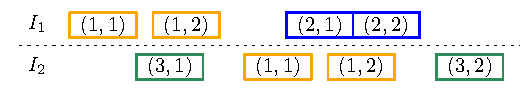
\includegraphics[width=0.7\textwidth]{figures/network_bilevel-1.pdf}
\end{figure}

\begin{itemize}
\item Lower-level trajectory optimization problem
\begin{itemize}
\item Direct transcription \(\rightarrow\) linear programming
\end{itemize}
\end{itemize}

\begin{figure}
  \centering
  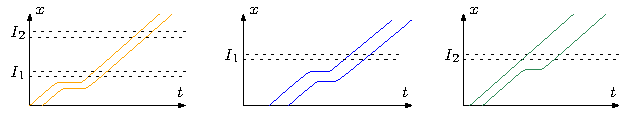
\includegraphics[width=0.8\textwidth]{figures/network_bilevel-2.pdf}
\end{figure}
\end{frame}
\begin{frame}[label={sec:org699a726}]{Determine crossing times}
\begin{tikzpicture}[remember picture, overlay]
\node[above=-7cm] at (current page.north)
{
  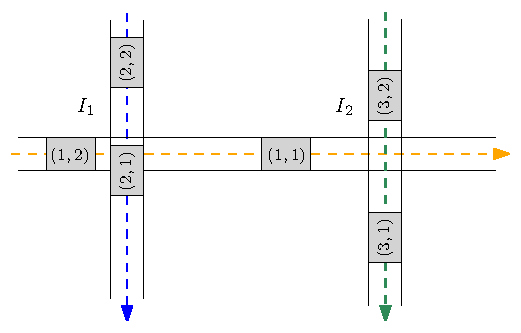
\includegraphics[width=0.7\textwidth]{figures/network_indices_1.pdf}
};
\end{tikzpicture}

\begin{tikzpicture}[remember picture, overlay]
\node[above=-9cm] at (current page.north)
{
  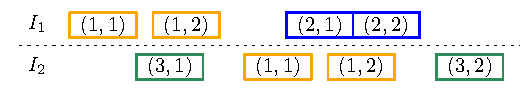
\includegraphics[width=0.8\textwidth]{figures/network_bilevel-1.pdf}
};
\end{tikzpicture}
\end{frame}
\begin{frame}[label={sec:org88a1565}]{Determine crossing order}
\begin{tikzpicture}[remember picture, overlay]
\node[above=-7cm] at (current page.north)
{
  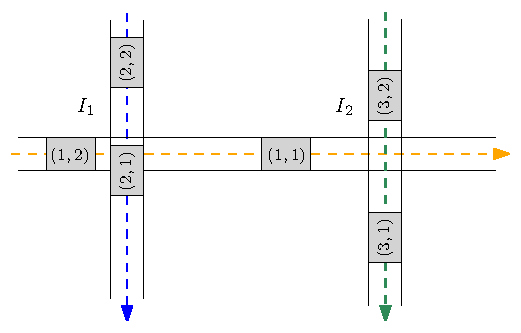
\includegraphics[width=0.7\textwidth]{figures/network_indices_1.pdf}
};
\end{tikzpicture}

\vspace{12em}

\begin{itemize}
\item Crossing times follow from crossing order
\end{itemize}
\end{frame}
\begin{frame}[label={sec:org6e24a98}]{Determine crossing order}
\begin{tikzpicture}[remember picture, overlay]
\node[above=-7cm] at (current page.north)
{
  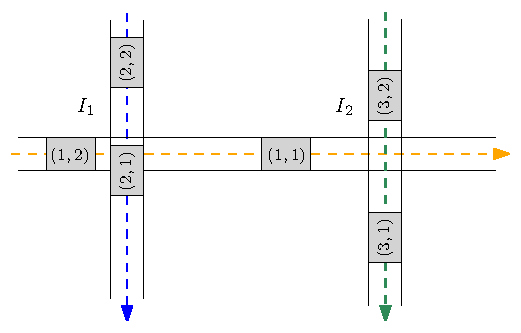
\includegraphics[width=0.7\textwidth]{figures/network_indices_1.pdf}
};
\end{tikzpicture}

\vspace{12em}

\begin{itemize}
\item Map instance to optimal crossing order
\item Use step-by-step construction\ldots{}
\end{itemize}
\end{frame}
\begin{frame}[label={sec:org53b0d1c}]{Determine crossing order}
\begin{figure}
  \centering
  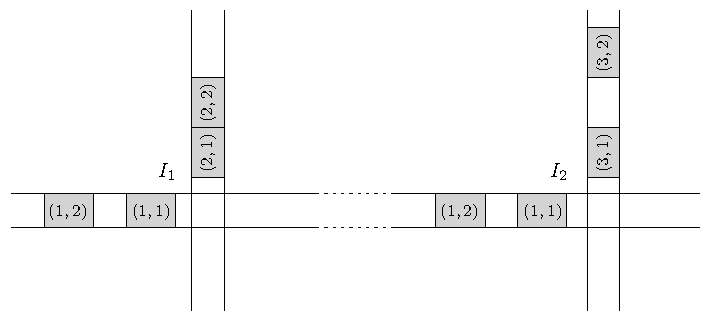
\includegraphics[width=0.9\textwidth]{figures/network_ordering-0.pdf}
\end{figure}
\end{frame}
\begin{frame}[label={sec:org04a3327}]{Determine crossing order}
\addtocounter{framenumber}{-1}
\begin{figure}
  \centering
  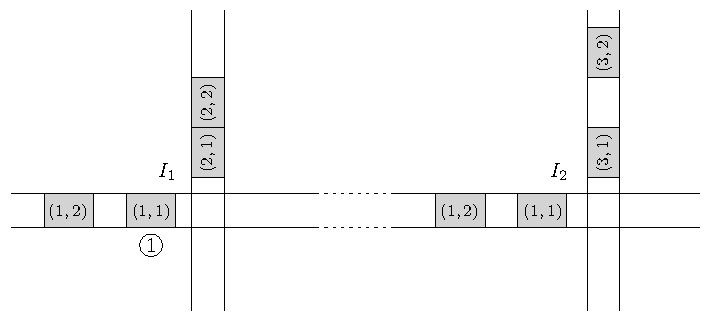
\includegraphics[width=0.9\textwidth]{figures/network_ordering-1.pdf}
\end{figure}
\end{frame}
\begin{frame}[label={sec:org2d4499b}]{Determine crossing order}
\addtocounter{framenumber}{-1}
\begin{figure}
  \centering
  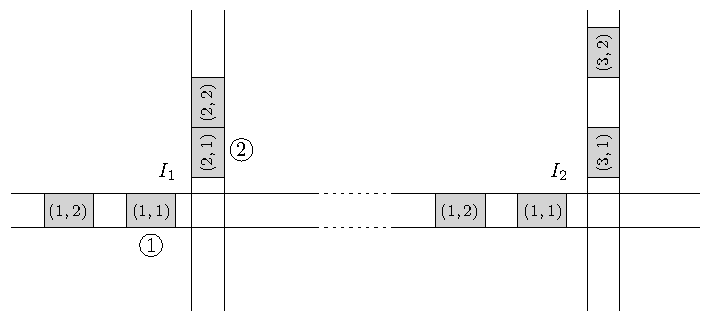
\includegraphics[width=0.9\textwidth]{figures/network_ordering-2.pdf}
\end{figure}
\end{frame}
\begin{frame}[label={sec:org258b8d4}]{Determine crossing order}
\addtocounter{framenumber}{-1}
\begin{figure}
  \centering
  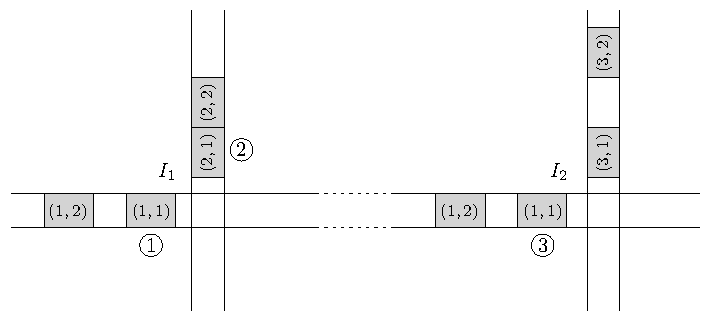
\includegraphics[width=0.9\textwidth]{figures/network_ordering-3.pdf}
\end{figure}
\end{frame}
\begin{frame}[label={sec:org7d05a17}]{Determine crossing order}
\addtocounter{framenumber}{-1}
\begin{figure}
  \centering
  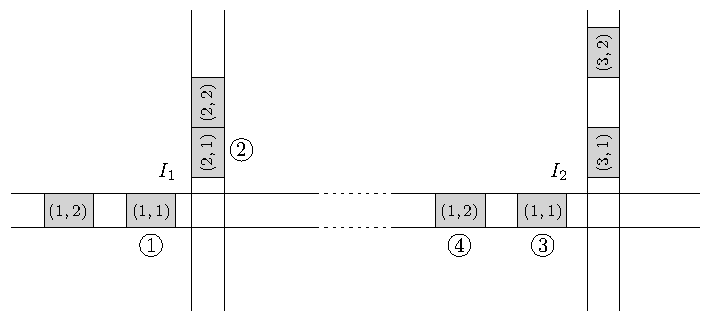
\includegraphics[width=0.9\textwidth]{figures/network_ordering-4.pdf}
\end{figure}
\end{frame}
\begin{frame}[label={sec:orgfde977c}]{Learn crossing order}
\begin{itemize}
\item \sout{Map instance to optimal crossing order}
\item Map partial order to next partial order (policy)

\(\vspace{0.1em}\)

\item We can learn this policy from examples!
\begin{itemize}
\item Imitation learning from optimal MILP solutions
\item Reinforcement learning with dense delay reward
\end{itemize}
\end{itemize}
\end{frame}
\begin{frame}[label={sec:org0da6232}]{Overview of project plan}
\begin{itemize}
\item Coordination as optimal control problem
\item Decompose: scheduling + trajectory optimization
\item Sequentially construct crossing order (policy)
\item Learn policy with imitation/reinforcement learning
\end{itemize}
\end{frame}
\begin{frame}[label={sec:org917ebbe}]{\(\;\)}
\begin{figure}
  \centering
  \href{https://github.com/jeroenvanriel/traffic-scheduling/blob/master/grid.gif}{
    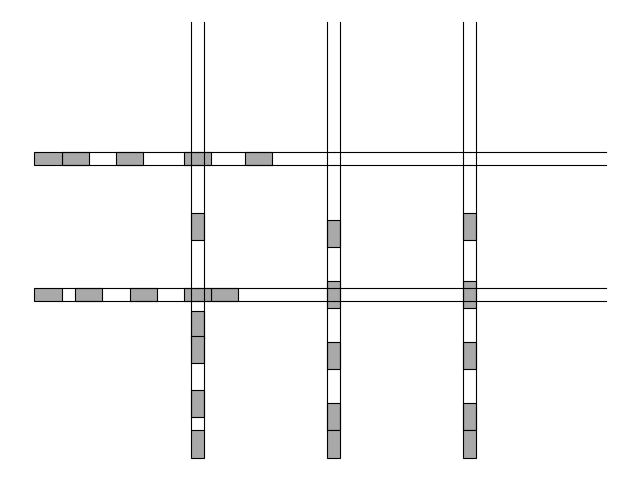
\includegraphics[width=0.7\textwidth]{figures/state_example.png}
  }
\end{figure}
\end{frame}
\begin{frame}[label={sec:org1fbd487}]{\(\;\)}
\centering
\color{structure}
\Large Appendix: Disjunctive graph
\normalsize
\vspace{2em}

\begin{columns}
\begin{column}{0.17\textwidth}
\end{column}

\begin{column}{0.83\textwidth}
\begin{itemize}

\end{itemize}
\end{column}
\end{columns}
\end{frame}
\begin{frame}[label={sec:orgf6f49cd}]{Disjunctive graph}
\begin{itemize}
\item Partial solutions encoded as disjunctive graph augmented with lower bounds on crossing times
\item Parameterize ordering policy based on graph neural network embedding of augmented disjunctive graph
\end{itemize}

\begin{figure}
  \centering
  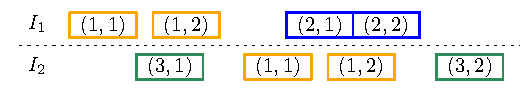
\includegraphics[width=0.8\textwidth]{figures/network_bilevel-1.pdf}
\end{figure}

\begin{figure}
  \centering
  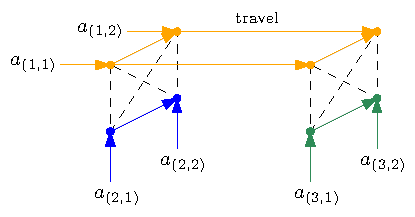
\includegraphics[width=0.7\textwidth]{figures/disjunctive_graph_variant.pdf}
\end{figure}
\end{frame}
\begin{frame}[label={sec:org4cb65af}]{Disjunctive graph}
\begin{itemize}
\item Partial solutions encoded as disjunctive graph augmented with lower bounds on crossing times
\item Parameterize ordering policy based on graph neural network embedding of augmented disjunctive graph
\end{itemize}

\begin{figure}
  \centering
  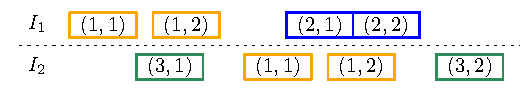
\includegraphics[width=0.8\textwidth]{figures/network_bilevel-1.pdf}
\end{figure}

\begin{figure}
  \centering
  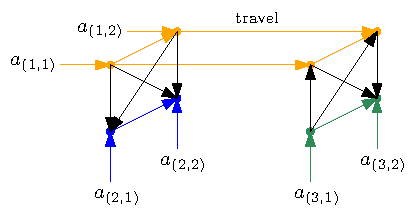
\includegraphics[width=0.7\textwidth]{figures/disjunctive_graph_complete.pdf}
\end{figure}
\end{frame}
\begin{frame}[label={sec:org9f2f8d4}]{\(\;\)}
\centering
\color{structure}
\Large Appendix: Related literature
\normalsize
\vspace{2em}

\begin{columns}
\begin{column}{0.17\textwidth}
\end{column}

\begin{column}{0.83\textwidth}
\begin{itemize}

\item Autonomous intersections
\item Neural combinatorial optimization

\end{itemize}
\end{column}
\end{columns}
\end{frame}
\begin{frame}[label={sec:orgdab9fd7}]{Autonomous intersections}
\begin{itemize}
\item ``Autonomous Intersection Control'' (Dresner \& Stone)
\begin{itemize}
\item Single intersection
\item Time slot reservation-based protocol
\item Central intersection manager
\end{itemize}
\end{itemize}

\begin{figure}
\centering
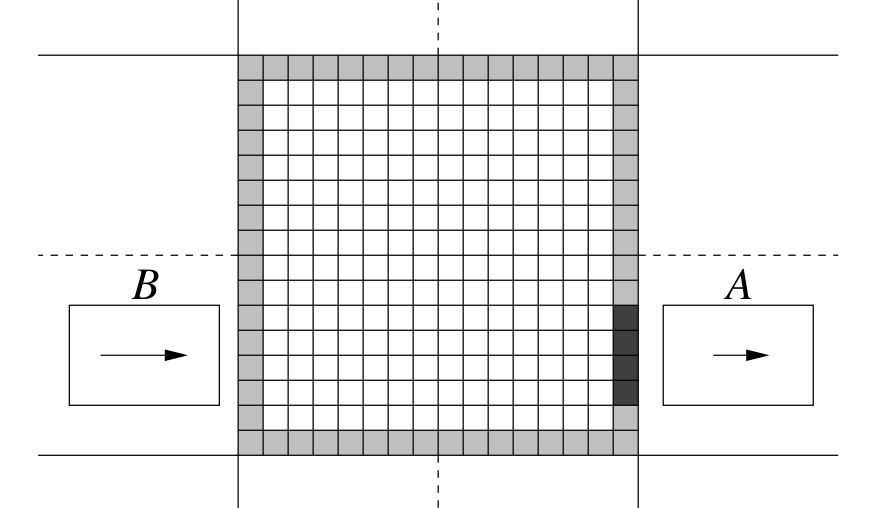
\includegraphics[width=0.6\textwidth]{figures/dresner_and_stone.png}
\end{figure}
\end{frame}
\begin{frame}[label={sec:orgeee3243}]{Autonomous intersections}
\begin{itemize}
\item ``Approximate Optimal Coordination'' (Hult et al.)
\begin{itemize}
\item Single intersection
\item Single vehicle per lane
\item Explicit collision-avoidance constraints
\end{itemize}
\end{itemize}

\begin{figure}
\centering
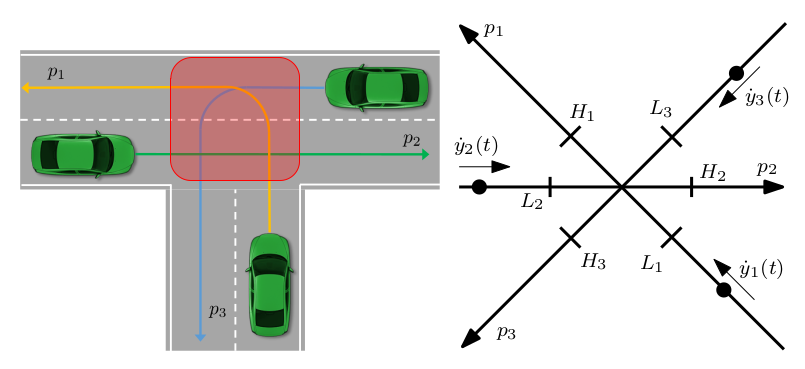
\includegraphics[width=0.7\textwidth]{figures/hult_et_al.png}
\end{figure}
\end{frame}
\begin{frame}[label={sec:org121cd3a}]{Neural combinatorial optimization}
\begin{itemize}
\item ``Learn to dispatch'' (Zhang et al.)
\begin{itemize}
\item Job-shop scheduling problem
\item Dispatch next operation
\item Policy using Graph Isomorphism Network (GIN)
\end{itemize}
\end{itemize}

\begin{figure}
  \centering
  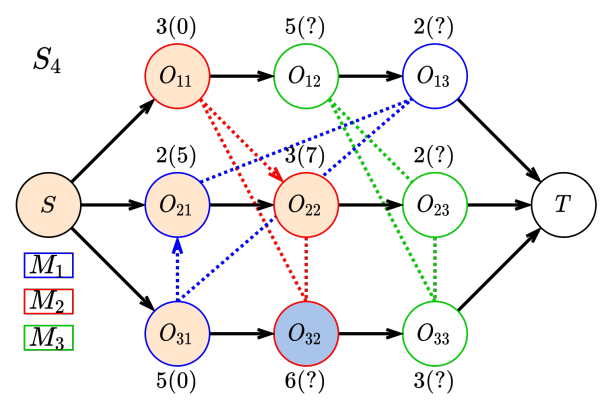
\includegraphics[width=0.5\textwidth]{../figures/Zhang-disjunctive-graph-s4.png}
\end{figure}
\end{frame}
\begin{frame}[label={sec:orgaf3d34f}]{\(\;\)}
\centering
\color{structure}
\Large Appendix: Single intersection
\normalsize
\vspace{2em}

\begin{columns}
\begin{column}{0.35\textwidth}
\begin{figure}
  \centering
  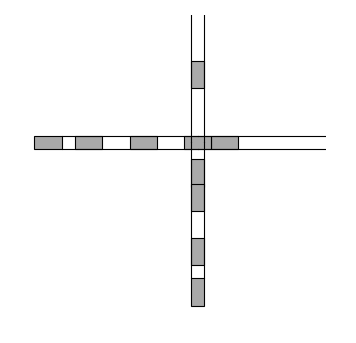
\includegraphics[width=1.0\textwidth]{../figures/single_intersection_example.png}
\end{figure}
\end{column}

\begin{column}{0.65\textwidth}
\begin{itemize}

\item Notation
\item Upper-level crossing time scheduling
\item Lower bound on starting times
\item Imitation learning with neural policy
\item Lower-level trajectory optimization

\end{itemize}
\end{column}
\end{columns}
\end{frame}
\begin{frame}[label={sec:orgd89b698}]{Notation}
\begin{itemize}
\item vehicle indices \(\mathcal{N}\)
\item \(y(i)\) is crossing time of vehicle \(i\)
\item \(r_i\) earliest crossing time of vehicle \(i\)
\end{itemize}

\begin{figure}
  \centering
  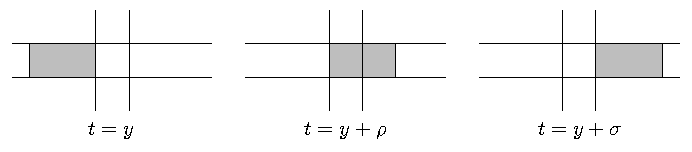
\includegraphics[width=0.9\textwidth]{figures/vehicle_crossing.pdf}
\end{figure}

\begin{itemize}
\item \(i\) and \(j\) same lane: \(y(i) + \rho \leq y(j)\)
\item \(i\) and \(j\) distinct lanes: \(y(i) + \sigma \leq y(j)\) or \(y(j) + \sigma \leq y(i)\)
\end{itemize}
\end{frame}
\begin{frame}[label={sec:orga8bc4d1}]{Upper-level crossing time scheduling}
\begin{itemize}
\item conjunctive constraints \(\mathcal{C}\)
\item disjunctive (conflict) constraints \(\mathcal{D}\)
\end{itemize}

\footnotesize
\begin{align*}
  \min_{y} \quad & \sum_{i \in \mathcal{N}} y(i) \\
  \text{ s.t. } \quad & r_{i} \leq y(i) ,  & \text{ for all } i \in \mathcal{N} ,\\
                    & y(i) + \rho \leq y(j) ,  & \text{ for all } (i,j) \in \mathcal{C} , \\
                    & y(i) + \sigma \leq y(j) \text{ or } y(j) + \sigma \leq y(i) , & \text{ for all } (i,j) \in \mathcal{D} \label{eq:disjunctions}
\end{align*}
\end{frame}
\begin{frame}[label={sec:orgc9e3197}]{Upper-level crossing time scheduling}
\begin{itemize}
\item Formulate as mixed-integer linear program (MILP)
\item Introduce binary decision variables \(\gamma_{ij}\)
\item Use big-M technique
\end{itemize}

\footnotesize
\begin{align*}
  \min_{y} \quad & \sum_{i \in \mathcal{N}} y_{i} & \\
  \text{s.t.} \quad & r_{i} \leq y_{i}, & \text{ for all } i \in \mathcal{N} , \\
  & y_{i} + \rho_{i} \leq y_{j}, & \text{ for all } (i,j) \in \mathcal{C} , \label{eq:conjunctions} \\
  & y_{i} + \sigma_{i} \leq y_{j} + \gamma_{ij}M, & \text{ for all } (i,j) \in {\mathcal{D}} , \\
  & y_{j} + \sigma_{j} \leq y_{i} + (1 - \gamma_{ij})M, & \text{ for all } (i,j) \in {\mathcal{D}} , \\
  & \gamma_{ij} \in \{0, 1\}, & \text{ for all } (i,j) \in {\mathcal{D}} \;
\end{align*}
\end{frame}
\begin{frame}[label={sec:org1ac697d}]{Lower bounds on starting times}
\begin{itemize}
\item Disjunctive graph given current order \(\pi\)
\item Nodes are vehicle indices \(\mathcal{N}\)
\item Edges \(i \xrightarrow{w(i,j)} j\)
\begin{itemize}
\item Conjunctive edges \(i \xrightarrow{\rho} j\)
\item Disjunctive edges \(i \xrightarrow{\sigma} j\) or \(j \xrightarrow{\sigma} i\)
\end{itemize}
\item Lower bounds \(\text{LB}_\pi\) on starting times given current order \(\pi\)
\end{itemize}
\begin{align*}
\text{LB}_\pi(j) = \max\{ r_j, \text{LB}_\pi(i) + w(i,j) \}
\end{align*}
\end{frame}
\begin{frame}[label={sec:org4f1b4cd}]{Imitation learning with neural policy}
\begin{figure}
  \centering
  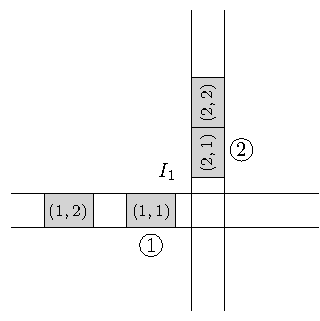
\includegraphics[width=0.4\textwidth]{figures/network_ordering-single.pdf}
\end{figure}

\begin{itemize}
\item crossing order \(\pi = ((1,1), (2,1))\) of vehicles
\item step-by-step construction of this order
\begin{itemize}
\item 1. choose \((1,1)\)
\item 2. choose \((2,1)\)
\item 3. \(\;\) \ldots{}
\end{itemize}
\end{itemize}
\end{frame}
\begin{frame}[label={sec:org7e4c43f}]{Imitation learning with neural policy}
\begin{itemize}
\item get optimal trajectories from MILP solver
\item parameterize policy based on \(\text{LB}_\pi\)
\begin{itemize}
\item only consider \(\text{LB}_\pi(j)\) for unscheduled \(j\)
\item recurrent embedding of \(\text{LB}_\pi(j)\) per lane
\item alternatively, use zero padding
\end{itemize}
\item fit policy parameters to expert transitions
\end{itemize}
\end{frame}
\begin{frame}[label={sec:orgb53b409}]{Lower-level trajectory optimization}
\begin{itemize}
\item position \(x\), velocity \(v\), control input \(u\)
\item position of vehicle in front \(x'\), follow distance \(L\)
\item position of intersection \(B\), crossing time \(\tau\)
\end{itemize}

\begin{align*}
  {\arg\min}_{x: [0, \tau] \rightarrow \mathbb{R}} & \int_{0}^{\tau} |x(t)| dt \\
  \text{ s.t. } & \ddot{x}(t) = u(t) , &  \text{ for all } t \in [0, \tau] , \\
  & |u(t)| \leq a_{\max} , &  \text{ for all } t \in [0, \tau] , \\
  & 0 \leq \dot{x}(t) \leq v_{\max} , &  \text{ for all } t \in [0, \tau] , \\
  & x'(t) - x(t) \geq L , &  \text{ for all } t \in [0, \tau] , \\
  & (x(0), \dot{x}(0)) = s_{0} , \\
  & (x(\tau), \dot{x}(\tau)) = (B, v_{\max})
\end{align*}
\end{frame}
\end{document}
